\documentclass[../master.tex]{subfiles}

\graphicspath{ {../images/} }
\begin{document}


\chapter{Introduction}

	\section{Motivation}\label{sec:motivation}
		The merit of a nuclear system simulation is heavily dependent on the accuracy of the input nuclear data. Nuclear data (such as cross sections, particle emissions, etc.) is often complicated and highly energy dependent, which poses a challenge for those interested in effcieiently simulating the behavior of a nuclear system. Nuclear data is released in ``evaluations'', which are prepared by statistically combining experimentally measured data with theoretical predictions. The most widely used format for these evaluations is called the Evaluated Nuclear Data File (ENDF)~\cite{endfManual}. ENDF files are generally not directly used by nuclear simulations, but are rather preprocessed to account for simulation-specific conditions. In doing so, the ENDF is converted into a more usable form, called ``a compact ENDF'' (ACE)~\cite{ace}.\par
		
		Currently, the most widely trusted code used for nuclear data preprocessing is NJOY, which has been developed and maintained at Los Alamos National Lab (LANL) since the early 1970's~\cite{njoy}. It has a large users base and is versatile for many nuclear data related tasks, including resonance reconstruction, Doppler-Broadening, multi-group cross section generation, and the preparation of thermal neutron scattering data. NJOY's capabilities are spread across 24 modules, each of which has a specified task. Two modules in particular, LEAPR and THERMR, handle the calculation and representation of thermal scattering from bound moderators. While the accuracy of thermal neutron scattering data can greatly dictate the quality of thermal reactor analysis and safety margin calculations, it remains a difficult problem, due to effects (molecular structure, neutron wavelength, described below) that are not apparent for higher neutron energies. \par

		Both thermal neutron scattering and resonant neutron scattering are highly dependent on incoming neutron energy. However, thermal neutron scattering cross sections must also account for molecular structure, since the energy of the incoming neutron is generally on the order of the molecules' excitation modes (i.e. below 1-10 eV). Excitation of these excitation modes can result in vibration, translation, or rotation of the target. Vibrational modes, also called phonons, are a primary concern when describing neutron scattering in a solid. In addition to the molecular excitation, thermal neutrons data processing is further complicated by considering the long neutron de Broglie wavelength. When a neutron has energy in the thermal region, its wavelength can be on the order of the interatomic spacing, which allows it to interact with multiple nuclei, as opposed to a single atom~\cite{jesseholmes}. 

		Despite the above complications, a thermal scattering relationship $S(\alpha,\beta,T)$ is constructed to relate unitless neutron momentum and energy exchange ($\alpha$ and $\beta$, respectively) with the double differential inelastic incoherent scattering cross section $\sigma\left(E\rightarrow E',\mu\right)$. Once $S(\alpha,\beta,T)$, also called the ``scattering law'', is obtained, the cross section can be obtained using

		\begin{equation}
			\sigma\left(E\rightarrow E',\mu\right)=\frac{\sigma_{b}}{2k_bT}\sqrt{\frac{E'}{E}}S(\alpha,\beta,T),\label{eq:sabDefinition}
		\end{equation}
		% A scattering relationship $S(\alpha,\beta,T)$ can be constructed to understand and quantify the behavior of these phonons, which for this text will be considered synonymous to a frequency spectrum of excitations. , which can be thought of as a coordinated wave of atomic vibrations. $S(\alpha,\beta,T)$ directly depends on the scattering neutron's change in energy, its change in momenum, and the scattering material's temperature~\cite{jesseholmes}.\par
		where $\sigma_b$ is the characteristic bound scattering cross section of the target isotope, and $k_b$ is Boltzmann's constant and $T$ is the temperature. As shown in Eq.~\ref{eq:sabDefinition}, if $S(\alpha,\beta,T)$ can be accurately obtained, the differential inelastic incoherent scattering cross section $\sigma\left(E\rightarrow E',\mu\right)$ is simple to calculate. Thus, the quality of thermal nuclear system modeling is directly tied to the preparation of the scattering law.

		% This project aims address the aforementioned insufficiencies in the preprocessing of thermal scattering nuclear data, while working in collaboration with NJOY developerrs at LANL. The scattering material's molecular structures must be accounted for and represented, while avoiding the limiting premature discretization step that is currently used. This would further allow for nuclear data processing codes to avoid discretization of the $S(\alpha,\beta,T)$ thermal scattering law that is used to describe and characterize thermal scattering behavior, thus allowing for legitimate and meaningful uncertianty quantification of the final processed nuclear data.


	\section{Current Methods of Preparing $S(\alpha,\beta,T)$}
		\subsection{Types of Thermal Neutron Scattering}
			As mentioned in Sec.~\ref{sec:motivation}, the most widely used code for nuclear data processing is NJOY, which through two of its modules (LEAPR and THERMR) has the ability to prepare thermal scattering data. In particular, LEAPR is used to create a $S(\alpha,\beta,T)$ table, while THERMR tabulates the scattering law into a convenient form for simulations to use. Since LEAPR primarily calculates $S(\alpha,\beta,T)$, it will be of primary focus for the rest of this section.\par

			Thermal neutron scattering can be broken into elastic and inelastic parts, which can then be further separated into coherent and incoherent parts. Elastic thermal scattering implies no change in neutron energy. Note that this differs from elastic scattering off of a single particle, in that a thermal neutron will elastically scatter off of an entire lattice, which makes the effective mass of the target extremely large. Thermal inelastic scattering can result in neutron energy loss, which corresponds to target excitation. At these low energies, neutron up-scattering can also occur, which implies neutron energy gain, and corresponds to target de-excitation. Excitations can correspond to creation of vibrational modes (phonons), as well as the creation of translational or rotational modes. For a system of particles with randomly distributed spins, coherent scattering consists of interacting wave effects, whereas incoherent scattering consists solely of a sum of non-interacting waves\footnote{Materials such as cold hydrogen that do not have randomly distributed have additional effects, so they have be considered apart from this simple coherent/incoherent discussion.}.\par

			% DO NOT DELETE THIS 
			% On pg. 16 of his thesis, Jesse Holmes states 
			% """ Incorporating the incoherent approximation is a common practice in the theoretical calculation of thermal neutron scattering kernels. It is physically valid in many nuclear engineering applications and it allows the calculation of cross sections to proceed analytically with ease. Cases where coherent interference in inelastic scattering is not negligible, such as for graphite, will be discussed separately in Sections 3.7.4 and 4.1."""
			% which confirms my fuzzy recollection that incoh approx = neglect inelastic coherent
			For materials with randomly distributed crystallites, the form of coherent inelastic scattering nearly equals that of incoherent inelastic scattering. This allows the coherent and incoherent inelastic components to be combined into one inelastic contribution, an approximation known as the ``incoherent approximation''~\cite{njoy,jesseholmes}. Thus, LEAPR separates the scattering calculation into inelastic, coherent elastic, and incoherent inelastic. This project focuses on inelastic scattering, due to the predominant importance of neutron energy change. 


		\subsection{Inelastic Thermal Neutron Scattering}
			Recall from Sec.~\ref{sec:motivation} that the double differential inelastic cross section is defined as 
			\begin{equation*}
				\sigma\left(E\rightarrow E',\mu\right)=\frac{\sigma_{b}}{2kT}\sqrt{\frac{E'}{E}}S_{n.sym}(\alpha,\beta,T)\tag{\ref{eq:sabDefinition}}
			\end{equation*}
			which describes a neutron with incoming energy $E$ scattering with cosine $\mu$ into energy $E'$. Recall again that $\sigma_b$ is the characteristic bound scattering cross section for the target, $k_b$ is Boltzmann's constant, and $T$ is the temperature. Note that $S_{n.sym}(\alpha,\beta,T)$ is the non-symmetric form of the scattering law, which will be further discussed in !!!!!!!!!!!!!!!!!!!. Dimensionless momentum and energy transfer, $\alpha$ and $\beta$ respectively, are defined as 
			\begin{equation}
				\alpha=\frac{E'+E-2\mu\sqrt{E'E}}{AkT}
			\end{equation}
			\begin{equation}
				\beta=\frac{E'-E}{kT}
			\end{equation}
			The symmetric scattering law $S_{n.sym}(\alpha,\beta)$ can be written as an integral across time in units of $\hbar/k_bT$ seconds, [THIS USES THE GAUSSIAN APPROXIMATION SO CHECK OUT Scattering of Slow Neutrons by a Liquid George H. Vineyard]
			\begin{equation}
				S_{n.sym}(\alpha,\beta,T)=\frac{1}{2\pi}\int_{-\infty}^{\infty}\mathrm{e}^{i\beta\hat{t}}\mathrm{e}^{-\gamma(\hat{t})}~d\hat{t}\label{eq:sabIntegralWithGamma}
			\end{equation}
			where 
			% \begin{equation} 
			% 	\gamma(\hat{t})=\alpha\int_{-\infty}^{\infty}P(\beta)\left[1-\mathrm{e}^{-i\beta\hat{t}}\right]\mathrm{e}^{-\beta/2}d\beta
			% \end{equation}

			% \begin{equation}
			% 	P(\beta)=\frac{\rho(\beta)}{2\beta\sinh(\beta/2)}
			% \end{equation}
			\begin{equation} 
				\gamma(\hat{t})=\alpha\int_{-\infty}^{\infty}P(\beta)\left[1-\mathrm{e}^{-i\beta\hat{t}}\right]\mathrm{e}^{-\beta/2}~d\beta\label{eq:gamma}
			\end{equation}
			and
			\begin{equation}
				P(\beta)=\frac{\rho(\beta)}{2\beta\sinh(\beta/2)}.
			\end{equation}
			Note that $\rho(\beta)$ is the phonon distribution or excitation frequency spectrum characteristic to the material, and that it normalizes to unity,
			\begin{equation}
				\int_{0}^{\infty}\rho(\beta)d\beta=1.
			\end{equation}
			Note that to get to this point, the only assumption made is that equating the form of incoherent inelastic scattering with that of coherent elastic scattering (incoheren approximation). At this point, LEAPR decomposes the frequency spectrum $\rho(\beta)$,
			\begin{equation}
				\rho(\beta)=\sum_{j=1}^{\#~\mbox{osc.}}\omega_j\delta(\beta_j)+\rho_s(\beta)+\rho_t(\beta))
			\end{equation}
			into a sum of discrete oscillators (represented by weighted delta-functions $\omega_j\delta(\beta_j)$), a solid-type spectrum $\rho_s(\beta)$, and a translational spectrum $\rho_t(\beta)$. The solid-type spectrum and translational spectrum integrate to $\omega_s$ and $\omega_t$, respectively, such that 
			\begin{equation}
				\sum_{j=1}^{\#~\mbox{osc.}}\omega_j + \omega_s + \omega_t = 1.
			\end{equation}
			LEAPR uses each component of this decomposed frequency distribution to create a corresponding scattering law $S_{sym,i}(\alpha,\beta,T)$, then convolves these individual scattering laws to retreive the true scattering relation $S_{n.sym}(\alpha,\beta,T)$.

			\subsubsection{Solid-Type Continuous Spectra}
				The solid-type continuous conribution to $S_{n.sym}(\alpha,\beta,T)$ can be calculated by representing Eq.~\ref{eq:sabIntegralWithGamma} as a sum, and using a finite number of terms of that sum to approximate a contribution value. The solid-type continuous spectra depends on the frequency distributino $\rho(\beta)$.
				Eq.~\ref{eq:gamma} can be rewritten as 
				\begin{equation} 
					\gamma(\hat{t})=\alpha\lambda_s-\alpha\int_{-\infty}^{\infty}P(\beta)\mathrm{e}^{-\beta/2}\mathrm{e}^{-i\beta\hat{t}}~d\beta.\label{eq:improvedGamma}
				\end{equation}
				where $\lambda_s$, known as the Debye-Waller coefficient for the solid-type spectra, is defined as 
				\begin{equation}
					\lambda_s = \int_{-\infty}^\infty P(\beta')e^{-\beta'/2}~d\beta'.
				\end{equation}
				Thus, the exponential of Eq.~\ref{eq:improvedGamma} is
				\begin{equation} 
					\mathrm{e}^{-\gamma(\hat{t})}=\sum_{n=0}^\infty\left(\mathrm{e}^{-\alpha\lambda_s}\frac{1}{n!}\left[\alpha\int_{-\infty}^{\infty}P(\beta')\mathrm{e}^{-\beta'/2}\mathrm{e}^{-i\beta'\hat{t}}~d\beta'\right]^n\right)
				\end{equation}
				where the exponential of the latter term has been represented as a Taylor series. The above can be used in Eq.~\ref{eq:sabIntegralWithGamma}, yielding
				\begin{align}
					S_{n.sym}(\alpha,\beta,T)=~&\frac{1}{2\pi}\int_{-\infty}^{\infty}\mathrm{e}^{i\beta\hat{t}}\sum_{n=0}^\infty\left(\mathrm{e}^{-\alpha\lambda_s}\frac{1}{n!}\left[\alpha\int_{-\infty}^{\infty}P(\beta')\mathrm{e}^{-\beta'/2}\mathrm{e}^{-i\beta'\hat{t}}~d\beta'\right]^n\right)~d\hat{t}\\
				% \end{align}
				% \begin{align}
					=~&\mathrm{e}^{-\alpha\lambda_s}\sum_{n=0}^\infty\frac{\alpha^n}{n!}\frac{1}{2\pi}\int_{-\infty}^{\infty}\mathrm{e}^{i\beta\hat{t}}\left[\int_{-\infty}^{\infty}P(\beta')\mathrm{e}^{-\beta'/2}\mathrm{e}^{-i\beta'\hat{t}}~d\beta'\right]^n~d\hat{t}\\
					% =~&\mathrm{e}^{-\alpha\lambda_{s}}\sum_{n=0}^{\infty}\frac{\alpha^n}{n!}\lambda_{s}^{n}\mathcal{T}_{n}(\beta)\\
					=~&\mathrm{e}^{-\alpha\lambda_{s}}\sum_{n=0}^{\infty}\frac{1}{n!}\left[\alpha\lambda_{s}\right]^{n}\mathcal{T}_{n}(\beta)\label{eq:sumToGetToContinSab}
				\end{align}
				where
				\begin{equation}
					\lambda_s^n\mathcal{T}_n(\beta)=\frac{1}{2\pi}\int_{-\infty}^{\infty}\mathrm{e}^{i\beta\hat{t}}\left[\int_{-\infty}^{\infty}P(\beta')\mathrm{e}^{-\beta'/2}\mathrm{e}^{-i\beta'\hat{t}}~d\beta'\right]^n~d\hat{t}.
				\end{equation}
				Note that
				\begin{equation}
					\mathcal{T}_0(\beta)=\delta(\beta)
				\end{equation}
				and
				\begin{align}
					\mathcal{T}_1(\beta)&=~\frac{1}{2\pi\lambda_s}\int_{-\infty}^\infty e^{i\beta\hat{t}}\int_{-\infty}^\infty P(\beta')e^{-\beta'/2}e^{-i\beta'\hat{t}}~d\beta'~d\hat{t}\\
					&=~\frac{1}{2\pi\lambda_s}\int_{-\infty}^\infty P(\beta')e^{-\beta'/2} \int_{-\infty}^\infty e^{i(\beta-\beta')\hat{t}}~d\hat{t}~d\beta'\\
					&=~\frac{1}{\lambda_s}\int_{-\infty}^\infty P(\beta')e^{-\beta'/2} \delta(\beta-\beta')~d\beta'\\
					&=~\frac{P(\beta)e^{-\beta/2}}{\lambda_s}.
				\end{align}
				As shown in Appendix~\ref{app:TnConvolutionDeriv}, $\mathcal{T}_n(\beta)$ can be attained using a convolution integral,
				\begin{equation}
					\mathcal{T}_{n}(\beta)=\int_{-\infty}^{\infty}\mathcal{T}_{1}\left(\beta^{\prime}\right)\mathcal{T}_{n-1}\left(\beta-\beta^{\prime}\right)d\beta^{\prime}\tag{\ref{ap:eq:finalTn}}.
				\end{equation}
				Solving the solid-type, continuous contribution to $S_{n.sym}(\alpha,\beta,T)$ can be done by computing $\mathcal{T}_i(\beta)$ for $i$ from 1 to a sufficiently large value of $n$. These $\mathcal{T}_i(\beta)$ values can be used in the Eq.~\ref{eq:sumToGetToContinSab}, which directly contributes to $S_{n.sym}(\alpha,\beta,T)$.



			\subsubsection{Discrete Oscillator}
				Shown in Fig.~\ref{fig:phononDist} is the phonon distribution for H in H$_2$O, as calculated by~\cite{phononModel}.
				\begin{figure}[h]
				    \centering
				    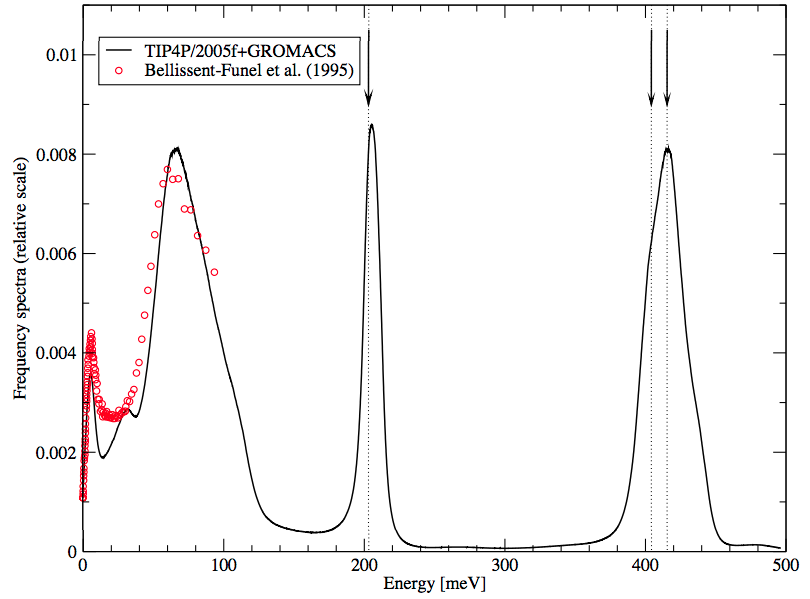
\includegraphics[width=0.6\textwidth]{images/HinH2OphononDist75.png}
				    \caption[Phonon Distribution for H in H$_2$O]{Phonon Distribution for H in H$_2$O~\cite{phononModel}. The red points and the arrows represent measured data against which to compare the calculated spectrum. Of particular interest are the two peaks near 200 and 400 meV, which are approximated in LEAPR as discrete oscillators.}
				    \label{fig:phononDist}
				\end{figure}
                                Often, vibrational modes appear as sharp peaks in the frequency distribution, and can be treated as a weighted delta function at energy $E$, $\omega_i\delta_i(E)$. The corresponding 
				\begin{equation}
					\mathcal{S}_{i}(\alpha,\beta)=\mathrm{e}^{-\alpha\lambda_{i}}\sum_{n=-\infty}^{\infty}\delta\left(\beta-n\beta_{i}\right)I_{n}\left[\frac{\alpha w_{i}}{\beta_{i}\sinh\left(\beta_{i}/2\right)}\right]\mathrm{e}^{-n\beta_{i}/2}
				\end{equation}
				\begin{equation}
					\mathcal{S}_{i}(\alpha,\beta)=\sum_{n=-\infty}^{\infty}A_{in}(\alpha)\delta\left(\beta-n\beta_{i}\right)
				\end{equation}
                                \begin{equation}
                                        \lambda_{i}=w_{i}\frac{\operatorname{coth}\left(\beta_{i}/2\right)}{\beta_{i}}
                                \end{equation}
                                where $\lambda_i$ is the Debye-Waller coefficient corresponding to the $i^{th}$ oscillator. When combining a continuous, solid-type spectrum with discrete oscillators, the total Debye-Waller coefficient is simply the sum,
                                \begin{equation}
                                        \lambda=\lambda_{s}+\sum_{i=1}^{N}\lambda_{i}
                                \end{equation}
                                where there are $N$ oscilllators considered.

%Polyatomic molecules normally contain a number of vibrational modes that can be represented as discrete oscillators. The distribu- tion function for one oscillator is given by wiδ(βi), where wi is the fractional weight for mode i, and βi is the energy-transfer parameter computed from the mode’s vibrational frequency. The corresponding scattering law is given by






			
			\subsubsection{Translational Spectra}

	\section{Areas of Improvement}
		\subsection{Input Phonon Distribution Approximations}

		\subsection{Sampling from $S(\alpha,\beta,T)$}

























\end{document}
